\documentclass[compress]{beamer}
\usepackage[francais]{babel}
\usepackage[latin1]{inputenc}
\usepackage{beamerthemesplit}
\usepackage[usenames,dvipsnames]{pstricks}
\usepackage{epsfig}
\usepackage{pst-grad} % For gradients
\usepackage{pst-plot} % For axes

\newcommand{\diapo}[2]{\frame{\frametitle{#1}#2}}
\newcommand{\imp}[1]{\textit{\textbf{#1}} }



\title{Carte de Kohonen}
\author{Hubert Godfroy}
\date{12 juin 2012}

\begin{document}

\frame{\titlepage}

\section[Plan]{}
\frame{\frametitle{Plan}\tableofcontents}

\section{Rappels}

\diapo{Rappels}{
\begin{itemize}
\item R�seau de neurones
	\begin{itemize}
	\item Fonction de transfert pour chaque neurone
	\item Relation entre les neurones
	\item Organisation du r�seau (couches)
	\end{itemize}
\item Apprentissage non-supervis�
	\begin{itemize}
	\item Le r�seau �volue seul en fonction des entr�es qui lui sont donn�es.
	\item 
	\end{itemize}
\end{itemize}
}

\diapo{Structure}{
	% !TEX root = ../presentation.tex

% Generated with LaTeXDraw 2.0.8
% Sat Jun 09 10:58:37 CEST 2012
% \usepackage[usenames,dvipsnames]{pstricks}
% \usepackage{epsfig}
% \usepackage{pst-grad} % For gradients
% \usepackage{pst-plot} % For axes
\scalebox{1} % Change this value to rescale the drawing.
{
\begin{pspicture}(0,-1.5)(10.129199,1.5)
\psframe[linewidth=0.04,dimen=outer](2.6,-0.7)(1.8,-1.5)
\psframe[linewidth=0.04,dimen=outer](1.4,-0.7)(0.6,-1.5)
\psframe[linewidth=0.04,dimen=outer](3.8,-0.7)(3.0,-1.5)
\psframe[linewidth=0.04,dimen=outer](5.0,-0.7)(4.2,-1.5)
\psframe[linewidth=0.04,dimen=outer](0.8,1.5)(0.0,0.7)
\psframe[linewidth=0.04,dimen=outer](2.0,1.5)(1.2,0.7)
\psframe[linewidth=0.04,dimen=outer](3.2,1.5)(2.4,0.7)
\psframe[linewidth=0.04,dimen=outer](4.4,1.5)(3.6,0.7)
\psframe[linewidth=0.04,dimen=outer](5.6,1.5)(4.8,0.7)
\psline[linewidth=0.04cm,linecolor=blue,arrowsize=0.05291667cm 2.0,arrowlength=1.4,arrowinset=0.4]{->}(1.6,0.7)(1.0,-0.7)
\psline[linewidth=0.04cm,linecolor=blue,arrowsize=0.05291667cm 2.0,arrowlength=1.4,arrowinset=0.4]{->}(0.4,0.7)(1.0,-0.7)
\psline[linewidth=0.04cm,linecolor=blue,arrowsize=0.05291667cm 2.0,arrowlength=1.4,arrowinset=0.4]{->}(0.4,0.7)(2.2,-0.7)
\psline[linewidth=0.04cm,linecolor=blue,arrowsize=0.05291667cm 2.0,arrowlength=1.4,arrowinset=0.4]{->}(0.4,0.7)(3.4,-0.7)
\psline[linewidth=0.04cm,linecolor=blue,arrowsize=0.05291667cm 2.0,arrowlength=1.4,arrowinset=0.4]{->}(0.4,0.7)(4.6,-0.7)
\psline[linewidth=0.04cm,linecolor=blue,arrowsize=0.05291667cm 2.0,arrowlength=1.4,arrowinset=0.4]{->}(1.6,0.7)(2.2,-0.7)
\psline[linewidth=0.04cm,linecolor=blue,arrowsize=0.05291667cm 2.0,arrowlength=1.4,arrowinset=0.4]{->}(1.6,0.7)(3.4,-0.7)
\psline[linewidth=0.04cm,linecolor=blue,arrowsize=0.05291667cm 2.0,arrowlength=1.4,arrowinset=0.4]{->}(1.6,0.7)(4.6,-0.7)
\psline[linewidth=0.04cm,linecolor=blue,arrowsize=0.05291667cm 2.0,arrowlength=1.4,arrowinset=0.4]{->}(2.8,0.7)(1.0,-0.7)
\psline[linewidth=0.04cm,linecolor=blue,arrowsize=0.05291667cm 2.0,arrowlength=1.4,arrowinset=0.4]{->}(2.8,0.7)(2.2,-0.7)
\psline[linewidth=0.04cm,linecolor=blue,arrowsize=0.05291667cm 2.0,arrowlength=1.4,arrowinset=0.4]{->}(2.8,0.7)(3.4,-0.7)
\psline[linewidth=0.04cm,linecolor=blue,arrowsize=0.05291667cm 2.0,arrowlength=1.4,arrowinset=0.4]{->}(2.8,0.7)(4.6,-0.7)
\psline[linewidth=0.04cm,linecolor=blue,arrowsize=0.05291667cm 2.0,arrowlength=1.4,arrowinset=0.4]{->}(4.0,0.7)(1.0,-0.7)
\psline[linewidth=0.04cm,linecolor=blue,arrowsize=0.05291667cm 2.0,arrowlength=1.4,arrowinset=0.4]{->}(4.0,0.7)(2.2,-0.7)
\psline[linewidth=0.04cm,linecolor=blue,arrowsize=0.05291667cm 2.0,arrowlength=1.4,arrowinset=0.4]{->}(4.0,0.7)(3.4,-0.7)
\psline[linewidth=0.04cm,linecolor=blue,arrowsize=0.05291667cm 2.0,arrowlength=1.4,arrowinset=0.4]{->}(4.0,0.7)(4.6,-0.7)
\psline[linewidth=0.04cm,linecolor=blue,arrowsize=0.05291667cm 2.0,arrowlength=1.4,arrowinset=0.4]{->}(5.2,0.7)(1.0,-0.7)
\psline[linewidth=0.04cm,linecolor=blue,arrowsize=0.05291667cm 2.0,arrowlength=1.4,arrowinset=0.4]{->}(5.2,0.7)(2.2,-0.7)
\psline[linewidth=0.04cm,linecolor=blue,arrowsize=0.05291667cm 2.0,arrowlength=1.4,arrowinset=0.4]{->}(5.2,0.7)(3.4,-0.7)
\psline[linewidth=0.04cm,linecolor=blue,arrowsize=0.05291667cm 2.0,arrowlength=1.4,arrowinset=0.4]{->}(5.2,0.7)(4.6,-0.7)
\put(7,-1.195){Couche d'entr�e}
\put(7 ,1.005){Carte de \textsc{Kohonen}}
\put(7 ,0.0050){Liaisons pond�r�es}
\end{pspicture} 
}


}

\diapo{Apprentissage}{
	\begin{itemize}
	\item Porte sur les neurones de la carte
	\item On rep�re le neurone \imp{vainqueur} qui est le plus "proche" de la couche d'entr�e au sens des poids.
	\item Ses poids sont modifi�s pour diminuer cette distance.
	\item Cette modification est propag�e aux neurones voisins du vainqueur.
	\end{itemize}
}

\section{Application}

\diapo{Application : ROC}{
	\begin{itemize}
	\item la couche d'entr�e est un agencement en 2 dimensions de neurone repr�sentant chacun un pixel de l'image.
	\item La carte de Kohonen est de dimension 2
	\item L'ensemble des poids d'un neurone de la carte peut �tre vu comme la moyenne des pixels ayant �t� vue par ce neurone. Chaque neurone est donc une moyenne d'image qu'il a rencontr�es.
	\end{itemize}
	\texttt{http://hurlebouc.github.com/kohonen/doc/inherits.html}
}

\diapo{Exemple}{
	\begin{figure}[htbp]
	\centering
	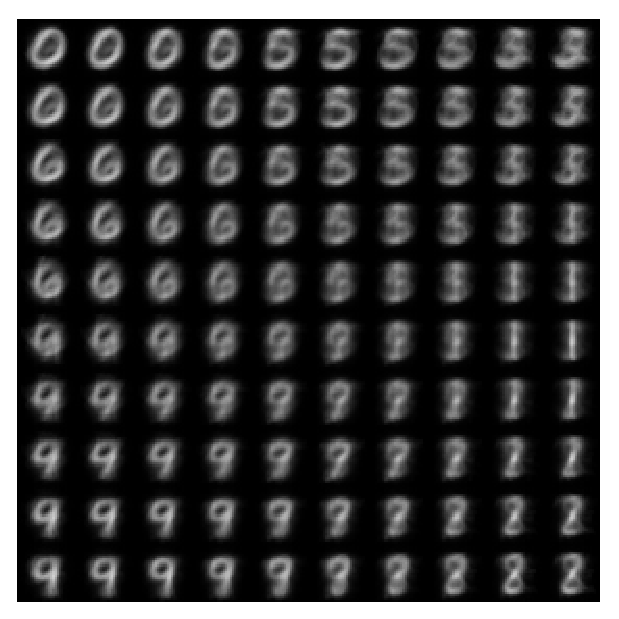
\includegraphics[width=5cm]{images/res.eps}
	\caption{Carte de \textsc{Kohonen} apr�s apprentissage}.
	\end{figure}
}

\section{Am�lioration}

\diapo{Discution}{
	
}



\end{document}
